\documentclass[sigconf]{acmart}
% \documentclass[sigconf,review]{acmart}\settopmatter{printfolios=true}

\usepackage{amssymb}
\usepackage{amsthm}
\usepackage{graphicx}
\usepackage{amsmath}
\usepackage{mathptmx}
\usepackage{mathtools}
\usepackage{stmaryrd}
\usepackage{adjustbox}
\usepackage{hyperref}
\usepackage{alltt}
\usepackage{url}
\usepackage{float}
\usepackage{minipage-marginpar}
\usepackage{style/utils}
\usepackage{style/code}
\usepackage{style/proof}
\usepackage{style/keywords}
\usepackage{style/layout}
\usepackage{style/judgements}

% for combinator pictures
\usepackage{tikz}
\usepackage{pgfplots}
\usetikzlibrary{shapes,arrows}

%\setcopyright{none}
\bibliographystyle{ACM-Reference-Format}
% \citestyle{acmauthoryear}

% -----------------------------------------------------------------------------
\begin{document}

\copyrightyear{2017}
\acmYear{2017}
\setcopyright{acmlicensed}
\acmConference{PPDP'17}{October 9--11, 2017}{Namur, Belgium}\acmPrice{15.00}\acmDOI{10.1145/3131851.3131865}
\acmISBN{978-1-4503-5291-8/17/10}

\begin{CCSXML}
<ccs2012>
<concept>
<concept_id>10003752.10003753.10003760</concept_id>
<concept_desc>Theory of computation~Streaming models</concept_desc>
<concept_significance>500</concept_significance>
</concept>
</ccs2012>
\end{CCSXML}


\renewcommand{\textrightarrow}{$\rightarrow$}

\ccsdesc[500]{Theory of computation~Streaming models}


\title{Machine Fusion}
\subtitle{Merging merges, more or less}

\author{Amos Robinson}
\affiliation{Ambiata and UNSW (Australia)}
\email{amosr@cse.unsw.edu.au}

\author{Ben Lippmeier}
\affiliation{Digital Asset and UNSW (Australia)}
\email{benl@ouroborus.net}

\makeatactive
\begin{abstract}
Compilers for stream programs often rely on a fusion transformation to convert the implied dataflow network into low-level iteration based code. Different fusion transformations handle different sorts of networks, with the distinguishing criteria being whether the network may contain splits and joins, and whether the set of fusible operators can be extended. We present the first fusion system that simultaneously satisfies all three of these criteria: networks can contain splits, joins, and new operators can be added to the system without needing to modify the overall fusion transformation.
\end{abstract}

\maketitle

\section{Introduction}
\label{s:Introduction}

Suppose we have two input streams of numeric identifiers, and wish to perform some analysis on them. The identifiers from both streams are sorted, but may include duplicates. We wish to produce an output stream of unique identifiers from the first input stream, as well as produce the unique union of both streams. Here is how we might write the source code, where @S@ is for @S@-tream.
\begin{code}
  uniquesUnion : S Nat -> S Nat -> (S Nat, S Nat)
  uniquesUnion sIn1 sIn2
   = let  sUnique = group sIn1
          sMerged = merge sIn1 sIn2
          sUnion  = group sMerged
     in   (sUnique, sUnion)
\end{code}

The @group@ operator detects groups of consecutive identical elements and emits a single representative, while @merge@ combines two sorted streams so that the output remains sorted. This example has a few interesting properties. Firstly, the data-access pattern of @merge@ is \emph{value-dependent}, meaning that the order in which @merge@ pulls values from @sIn1@ and @sIn2@ depends on the values themselves.
%: at each step, @merge@ must compare the values from both streams, and choose the stream with the smaller value to pull from.

Secondly, although @sIn1@ occurs twice in the program, at runtime we only want to handle its elements once. To achieve this, the compiled program must coordinate between the two uses of @sIn1@, so that a new value is read only when both @group@ and @merge@ are ready to receive it. Finally, as the stream length is unbounded, we cannot buffer arbitrarily many elements, or we risk running out of memory.

% To implement this program we might write each operator as its own concurrent process, sending stream elements over inter-process channels.
To implement this we might translate each operator into its own process in a concurrent network. This could be easy or hard, depending on the available language features for concurrency. However, the \emph{performance tuning} of such a system, such as using back-pressure to prevent buffers from being overrun, or how to chunk stream data to amortize communication overhead, is invariably a headache.

Instead, we would prefer to use \emph{stream fusion}, which is a program transformation that takes the implied dataflow network and produces a simple sequential loop that does not require extra process-control abstractions or unbounded buffering. Sadly, existing stream fusion transformations cannot handle our example.

As observed by \citet{kay2009you}, both pull and push fusion have fundamental limitations. Pull systems such as short-cut stream fusion~\cite{coutts2007stream} cannot handle cases where a stream is used by multiple consumers. We refer to this situation as a \mbox{\emph{split} --- in } our example the input stream @sIn1@ is split into both the @group@ and @merge@ consumers. Push systems such as foldr/build fusion~\cite{gill1993short} cannot fuse our example either, because they do not support operators with multiple inputs. We refer to this as a \emph{join} --- in our example the @merge@ operator expresses a join. Some systems support both: data flow inspired array fusion using series expressions~\cite{lippmeier2013data} allows both splits and joins but only for a limited, predefined set of operators. More recent work on polarized data flow fusion~\cite{lippmeier2016polarized} \emph{is} able to fuse our example, but requires the program to be rewritten to use explicitly polarized stream types.

In this paper we present Machine Fusion, a new approach. Each operator is expressed as a sequential imperative program which \emph{pulls} from input streams, and \emph{pushes} to output streams. We view each operator as a process in a concurrent process network. Our fusion transform then \emph{sequentializes} the concurrent process network into a single process, by choosing a particular interleaving of the operator code that requires no unbounded intermediate buffers. When fusion succeeds we know it has worked. There is no need to inspect the compiled code to debug poor performance, which is a common problem in systems based on general purpose transformations \cite{lippmeier2012:guiding}.

In summary, we make the following contributions:
\begin{itemize}
\item a process calculus for infinite streaming programs (\S\ref{s:Processes});
\item a fusion algorithm, the first to support splits and joins (\S\ref{s:Fusion});
\item benchmarks showing significant performance gains (\S\ref{s:Evaluation});
\item proof of soundness for the fusion algorithm in Coq (\S\ref{s:Proofs}).
\end{itemize}

Our fusion transform for infinite stream programs also serves as the basis for an \emph{array} fusion system, using a natural extension to finite streams. We discuss this extension in \S\ref{s:Finite}.


% BL: This is now discussed in S2.5 Breaking It Down.
% We might instead define a uniform sequential interface for data sources, with a single `pull' function that provides the next value in each stream. Each operator could be given this interface, so that values from each stream are computed on demand. This approach is commonly taken in database systems \cite{Graefe:Volcano}. However, this `pull' model does not support operators with multiple outputs, such as our example, at least not without unbounded buffering. Suppose a consumer pulls many elements from the @sUnique@ output stream. In order to perform the @group@ operation, the implementation needs to pull the corresponding source elements from the @sIn1@ input stream \emph{as well} as buffering an arbitrary number of them. It needs to buffer these elements because they are also needed to perform the @merge@ operation. When a consumer finally pulls from @sUnion@ we will be able to drain the buffer of @sIn1@ elements, but not before.

% TODO: move to related work.
% The polyhedral array fusion model~\cite{feautrier2011polyhedron} is used for loop transformations in imperative programs, but is based around affine loops, which makes it difficult to support value-dependent operators  such as @group@ and @merge@.

% -----------------------------------------------------------------------------
\section{Processes and Machines}
\label{s:Processes}

A \emph{process} in our system is a simple imperative program with a local heap. A process pulls source values from an arbitrary number of input streams and pushes result values to at least one output stream. The process language is an intermediate representation we use when fusing the overall dataflow network. When describing the fusion transform we describe the control flow of the process as a state machine, hence Machine Fusion. 

A \emph{combinator} is a template for a process which parameterizes it over the particular input and output streams, as well as values of configuration parameters such as the worker function used in a @map@ process. Each process implements a logical \emph{operator} --- so we use ``operator'' when describing the values being computed, but ``process'' and ``machine'' when referring to the implementation. 


% -----------------------------------------------------------------------------
\subsection{Grouping}

The definition of the @group@ combinator which detects groups of successive identical elements in the input stream is given in Figure~\ref{fig:Process:Group}. The process emits the first value pulled from the stream and every value that is different from the last one that was pulled. For example, when executed on the input stream @[1,2,2,3]@, the process will produce the output @[1,2,3]@. We include the concrete representation and a diagram of the process when viewed as a state machine.

The @group@ combinator has two parameters, @sIn1@ and @sOut1@, which bind the input and output streams respectively. The \emph{nu-binders} \mbox{($\nu$ @(f: Bool) (l: Nat)@...)} indicate that each time the @group@ combinator is instantiated, fresh names must be given to @f@, @l@ and so on, that do not conflict with other instantiations. Overall, the @f@ variable tracks whether we are dealing with the first value from the stream, @l@ holds the last value pulled from the stream (or 0 if none have been read yet), and @v@ holds the current value pulled from the stream. 

The body of the combinator is a record that defines the process. The @ins@ field defines the set of input streams and the @outs@ field the set of output streams. The @heap@ field gives the initial values of each of the local variables. The @instrs@ field contains a set of labeled instructions that define the program, while the @label@ field gives the label of the initial instruction. In this form, the output stream is defined via a parameter, rather than being the result of the combinator, as in the representation of @uniquesUnion@ from \S\ref{s:Introduction}. 

The initial instruction @(pull sIn1 v A1 [])@ pulls the next element from the stream @sIn1@, writes it into the heap variable @v@ (value), then proceeds to the instruction at label @A1@. The empty list @[]@ after the target label @A1@ can be used to update heap variables, but as we do not need to update anything yet we leave it empty. 

Next, the instruction @(case (f || (l /= v)) A2 [] A3 [])@ checks whether predicate @(f || (l /= v))@ is true; if so it proceeds to the instruction at label @A2@, otherwise it proceeds to @A3@. We use the variable @l@ (last) to track the last value read from the stream, and the boolean @f@ (first) to track whether this is the first element.

% AR: Clumsy, but added "at L2 executes:" to force @(push...)@ onto its own line. Otherwise it goes off the right.
When the predicate is true, the instruction at label @A2@ executes
@(push sOut1 v A3 [ l = v, f = F ])@
which pushes the value @v@ to the output stream @sOut1@ and proceeds to the instruction at label @A3@, once the variable @l@ is set to @v@ and @f@ to @F@ (False).

Finally, the instruction @(drop sIn1 A0 [])@ signals that the current element that was pulled from stream @sIn1@ is no longer required, and goes back to the first instruction at @A0@. 


\begin{figure*}

\begin{minipage}{0.6\textwidth}
\begin{alltt}
 group 
   = \(\lambda\) (sIn1: Stream Nat) (sOut1: Stream Nat). 
     \(\nu\) (f: Bool) (l: Nat) (v: Nat) (A0..A3: Label).
\end{alltt}
\begin{code}
     process
      { ins:    { sIn1  }
      , outs:   { sOut1 }
      , heap:   { f = T, l = 0, v = 0 }
      , label:  A0
      , instrs: { A0 = pull sIn1 v          A1 []
                , A1 = case (f || (l /= v)) A2 []  A3 []
                , A2 = push sOut1 v         A3 [ l = v, f = F ]
                , A3 = drop sIn1            A0 [] } }
\end{code}
\end{minipage}
\begin{minipage}{0.29\textwidth}
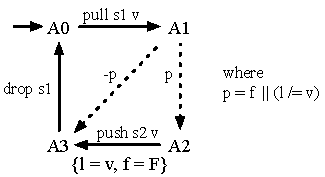
\includegraphics[scale=1.0]{figures/state-group.pdf}
\end{minipage}

\caption{The group combinator}
\label{fig:Process:Group}
\end{figure*}


% -----------------------------------------------------------------------------
\subsection{Merging}
\begin{figure*}
\begin{alltt}
       merge
         = \(\lambda\) (sIn1: Stream Nat) (sIn2: Stream Nat) (sOut2: Stream Nat). 
           \(\nu\) (x1: Nat) (x2: Nat) (B0..E2: Label).
\end{alltt}
\begin{code}
           process
            { ins:    { sIn1, sIn2 }
            , outs:   { sOut2 }
            , heap:   { x1 = 0, x2 = 0 }
            , label:  B0
            , instrs: { B0 = pull sIn1  x1   B1 []             , B1 = pull sIn2  x2   C0 []
                      , C0 = case (x1 < x2)  D0 []  E0 []      , D0 = push sOut2 x1   D1 []
                      , D1 = drop sIn1       D2 []             , D2 = pull sIn1  x1   C0 []
                      , E0 = push sOut2 x2   E1 []             , E1 = drop sIn2       E2 []
                      , E2 = pull sIn2 x2    C0 [] } }
\end{code}
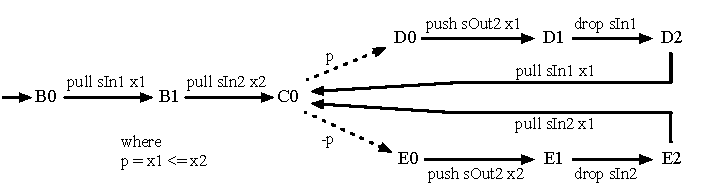
\includegraphics[scale=1.0]{figures/state-merge.pdf}
\caption{The merge combinator}
\label{fig:Process:Merge}
\end{figure*}

The definition of the @merge@ combinator, which merges two input streams, is given in Figure~\ref{fig:Process:Merge}. The combinator binds the two input streams to @sIn1@ and @sIn2@, while the output stream is @sOut2@. The two heap variables @x1@ and @x2@ store the last values read from each input stream. The process starts by pulling from each of the input streams. It then compares the two pulled values, and pushes the smaller of the values to the output stream. The process then drops the stream which yielded the the smaller value, then pulls from the same stream so that it can perform the comparison again.


% -----------------------------------------------------------------------------
\subsection{Fusion}

Our fusion algorithm takes two processes and produces a new one that computes the output of both. For example, suppose we need a single process that produces the output of the first two lines of our @uniquesUnion@ example back in \S\ref{s:Introduction}. The result will be a process that computes the result of both @group@ and @merge@ as if they were executed concurrently, where the first input stream of the @merge@ process is the same as the input stream of the @group@ process. In our informal description of the fusion algorithm we will instantiate the parameters of each combinator with arguments of the same names.

% -----------------------------------------------------------------------------
\subsubsection{Fusing Pulls}
\label{s:Fusion:FusingPulls}

The algorithm proceeds by considering pairs of states: one from each of the source process state machines to be fused. Both the @group@ machine and the @merge@ machine pull from the same stream as their initial instruction, so we have the situation shown in the top of Figure~\ref{fig:Fusion:Pulls}. The @group@ machine needs to transition from label @A0@ to label @A1@, and the @merge@ machine from @B0@ to @B1@. In the result machine we produce three new instructions that transition between four joint result states, @F0@ to @F3@.
Each of the joint result states represents a combination of two source states, one from each of the source machines. For example, the first result state @F0@ represents a combination of the @group@ machine being in its initial state @A0@ and the @merge@ machine being in its own initial state @B0@. 

We also associate each of the joint result states with a description of whether each source machine has already pulled a value from each of its input streams. For the @F0@ case at the top of Figure~\ref{fig:Fusion:Pulls} we have ((A0, \{sIn1 = none\}), (B0, \{sIn1 = none, sIn2 = none\})). The result state @F0@ represents a combination of the two source states @A0@ and @B0@. As both @A0@ and @B0@ are the initial states of their respective machines, those machines have not yet pulled any values from their two input streams, so both `sIn1' and `sIn2' map to `none'.

From the result state @F0@, both of the source machines then need to pull from stream @sIn1@, the @group@ machine storing the value in a variable @v@ and the @merge@ machine storing it in @x1@. In the result machine this is managed by first storing the pulled value in a fresh, shared buffer variable @b1@, and then using later instructions to copy the value into the original variables @v@ and @x1@. To perform the copies we attach updates to a @jump@ instruction, which otherwise transitions between states without affecting any of the input or output streams.

Finally, note that in the result states @F0@ through @F3@, the state of the input streams transitions from `none', to `pending' then to `have'. The `none' state means that we have not yet pulled a value from the associated stream. The `pending' state means we have pulled a value into the stream buffer variable (@b1@ in this case). The `have' state means that we have copied the pulled value from the stream buffer variable into the local variable used by each machine. 

% BL: Dropped this to fix pagination.
% In Figure~\ref{fig:Fusion:Pulls},  `sIn1' is set to `have' for the first machine in @F2@ after we have set `v = b1', while `sIn1' is set to `have' for the second machine in @F3@ after we have set `x1 = b1'. 


% -----------------------------------------------------------------------------
\subsubsection{Fusing Cases}
Once the result machine has arrived at the joint state @F3@, this is equivalent to the two source machines arriving in states @A1@ and @B1@ respectively. The lower half of Figure~\ref{fig:Fusion:Case} shows the next few transitions of the source machines. From state @A1@, the @group@ machine needs to perform a @case@ branch to determine whether to push the current value it has from its input stream @sIn1@ to output stream @sOut1@, or to just pull the next value from its input. From state @B1@, the @merge@ machine needs to pull a value from its second input stream @sIn2@. In the result machine, @F3@ performs the case analysis from @A1@, moving to either @F4@ or @F5@, corresponding to @A2@ and @A3@ respectively. From state @F4@, the push at @A2@ is executed and moves to @F5@, corresponding to @A3@. Finally, at @F5@ the @merge@ machine pulls from @sIn2@, moving from @F5@ to @F6@, corresponding to @B1@ and @C0@ respectively. As the stream @sIn2@ is only pulled from by the @merge@ machine, no coordination is required between the @merge@ and @group@ machines for this pull.


% -----------------------------------------------------------------------------
\subsection{Fused Result}

Figure~\ref{fig:Process:Fused} shows the final result of fusing @group@ and @merge@ together. There are similar rules for handling the other combinations of instructions, but we defer the details to \S\ref{s:Fusion}. The result process has two input streams, @sIn1@ and @sIn2@, and two output streams: @sOut1@ from @group@, and @sOut2@ from @merge@. The shared input @sIn1@ is pulled by @merge@ instructions at two places, and since both of these need to agree with when @group@ pulls, the @group@ instructions are duplicated at @F3@-@F5@ and @F13@-@F15@. The first set of instructions could be simplified by constant propagation to a single @push@, as @f@ is initially true.

To complete the implementation of our example from \S\ref{s:Introduction} we would now fuse this result process with a process from the final line of the example (also a @group@). Note that although the result process has a single shared heap, the heap bindings from each fused process are guaranteed not to interfere, as when we instantiate combinators to create source processes we introduce fresh names. 

% AR: Cut to make room for explanation why two copies of group pull
% The order in which pairs of processes are fused together does matter, as does the order in which instructions are interleaved --- we discuss both points further in \S\ref{s:FusionOrder} and \S\ref{s:Evaluation}.

% -----------------------------------------------------------------------------
\subsection{Breaking It Down}
We started with a pure functional program in \S\ref{s:Introduction}, reimagined it as a dataflow graph, then interleaved imperative code that implemented two of the operators in that dataflow graph. We needed to \emph{break down} the definition of each operator into imperative statements so that we could interleave their execution appropriately. We do this because the standard, single-threaded evaluation semantics of functional programs does not allow us to evaluate stream programs that contain both splits and joins in a space efficient way. Returning to the definition of @uniquesUnion@ from \S\ref{s:Introduction}, we cannot simply execute the @group@ operator on its entire input @sIn1@ before executing the @merge@ operator, as that would require us to buffer all data read from @sIn1@. Instead, during fusion we perform the job of a concurrent scheduler at compile time. In the result process the flow of control alternates between the instructions for both the @group@ and @merge@ operators, but as the instructions are interleaved directly there is no overhead due to context switching --- as there would be in a standard concurrent implementation using multiple threads.

The general approach of converting a pure functional program to a dataflow graph, then interleaving imperative statements that implement each operator was also used in prior work on Flow Fusion~\cite{lippmeier2013data}. However, in contrast to Flow Fusion and similar systems, with \mbox{Machine Fusion} we do not need to organize statements into a fixed \emph{loop anatomy} --- we simply merge them as they are. This allows us to implement a wider range of operators, including ones with nested loops that work on segmented streams.

Note that relying on lazy evaluation for @uniquesUnion@ does not eliminate the need for unbounded buffering. Suppose we converted each of the streams to lazy lists, and used definitions of @group@ and @merge@ that worked over these lists. As @uniquesUnion@ returns a pair of results, there is nothing preventing a consumer from demanding the first list (@sUnique@) in its entirety before demanding any of the elements from the second list (@sUnion@). If this were to happen then the runtime implementation would need to retain all elements of @sIn1@ before demanding any of @sIn2@, causing a space leak. Lazy evaluation is \emph{pull only} meaning that evaluation is driven by the consumer. The space efficiency of our fused program relies critically on the fact that processes can also \emph{push} their result values directly to their consumers, and that the consumers cannot defer the handling of these values.

% TODO: Blend this in.
% Note that we could construct the fused result machine in several ways. One option is to perform the case branch first and then pull from @sIn2@, another is to pull from @sIn2@ first and then perform the branch. By construction, the predicate used in the branch refers only to variables local to the @group@ machine, and the pull instruction from @B1@ stores its result in a variable local to the @merge@ machine. As the set of variables does not overlap, either ordering is correct. For this example we choose to perform the branch first, though will discuss the ramifications of this choice further in \S\ref{s:FusionOrder}. 

% TODO: Shift this later.
% As the @merge@ process merges infinite streams, if we execute it with a finite input prefix, it will arrive at an intermediate state that may not yet have pushed all available output. For example, if we execute the process with the input streams @[1,4]@ and @[2,3,100]@ then the values @[1,2,3,4]@ will be pushed to the output. After pushing the last value @4@, the process will block at instruction @E2@, waiting for the next value to become available from @sIn2@. We discuss how to handle finite streams later in ~\S\ref{s:Finite}.

% TODO: Talk about what drop is really for later.
% This @drop@ instruction is used to coordinate concurrent processes when performing fusion. The next element of a stream may only be pulled after all consumers of that stream have pulled and then and dropped the current element.

% -----------------------------------------------------------------------------
\begin{figure*}
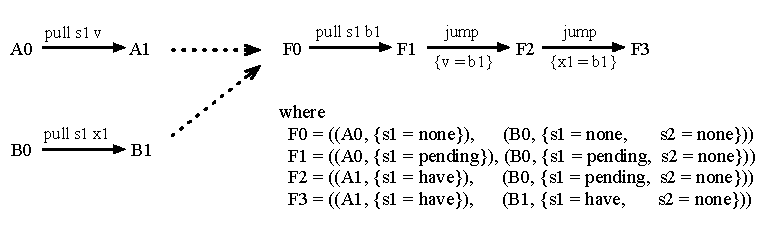
\includegraphics[scale=1.1]{figures/fuse-pull-pull.pdf}

\vspace{2em}

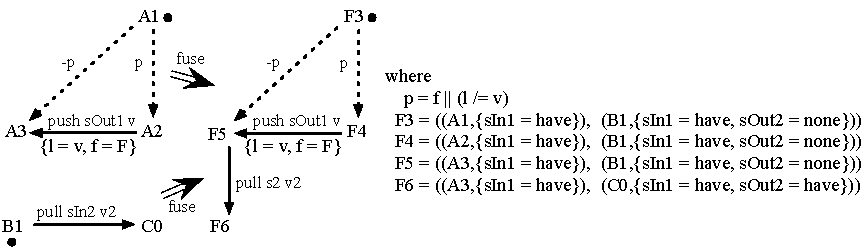
\includegraphics[scale=1.1]{figures/fuse-case-pull.pdf}
\caption{Fusing pull (top) and case (bottom) instructions}
\label{fig:Fusion:Pulls}
\label{fig:Fusion:Case}
\end{figure*}

% BL: Merged these figures togather to save space.
% \begin{figure*}
% \caption{Fusing case instructions}
% \label{fig:Fusion:Case}
% \end{figure*}

%%% AR: would like to highlight which machine is performing the current instruction, eg bolding "A0" when it's group moving from A0 to A1
\begin{figure*}
\definecolor{groupc}{HTML}{308030}
\definecolor{mergec}{HTML}{800000}
\definecolor{sharec}{HTML}{000080}

\newcommand\annot[5]{
  \tiny ((#1,   \> \tiny \{sIn1 =      #2\}), 
                \> \tiny (#3, \> \tiny \{sIn1 =      #4, \> \tiny sIn2 =      #5\}))
}

\newcommand\icase[7]{
 \tt{#1} \> \tt{= #2} \> \tt{#3} \> \tt{[ #4 ]} \> \tt{#5} \> \tt{[ #6 ]} \> \tiny #1 \> \tiny = #7
}

\newcommand\instr[5]{
 \tt{#1}\>\tt{= #2} \> \tt{#3} \> \tt{[ #4 ]} \> \> \> \tiny #1 \> \tiny = #5
}

\newcommand\tctt[2]{\textcolor{#1}{\tt{#2}}}

\hspace{5em}

\begin{adjustbox}{minipage=0.8\textwidth,margin=0pt \smallskipamount,center}
\begin{alltt}
process
\string{ ins:    \string{ \tctt{sharec}{sIn1},  \tctt{mergec}{sIn2} \string}
, outs:   \string{ \tctt{groupc}{sOut1}, \tctt{mergec}{sOut2} \string}
, heap:   \string{ \tctt{groupc}{f = T, l = 0, v = 0}, \tctt{mergec}{x1 = 0, x2 = 0}, \tctt{sharec}{b1 = 0} \string}
, label:  \tctt{sharec}{F0}
\end{alltt}

\begin{tabbing}
@  @ \=
@, F17@  \= = @case (f || (l /= v)) @
         \= @F17@ \= @[ ]     @ \= @F17@ \= @[ ]@
@   @ \= \tiny @   @F17 \= \tiny = ((A0, \= \tiny \{sIn1 = pending\}), \= \tiny (B0, \= \tiny \{sIn1 = pending, \= \tiny sIn2 = pending\})) \kill

@, instrs:@

% I have no idea how this works, but you need this particular incantation to colour the whole line in a tabbing environment.
% It's not ideal that the { and , are coloured too, but that can't be helped.
\\[0pt \color{sharec}]
\> @{@
\instr{F0}{pull sIn1 b1}{F1}{}
      {\annot{A0}{none}{B0}{none}{none}}

\\[0pt \color{groupc}]
\> @,@
\instr{F1}{jump}{F2}{v  = b1}
      {\annot{A0}{pending}{B0}{pending}{none}}

\\[0pt \color{mergec}]
\> @,@
\instr{F2}{jump}{F3}{x1 = b1}
      {\annot{A1}{have}{B0}{pending}{none}}

\\[0pt \color{groupc}]
\> @,@
\icase{F3}{case (f || (l /= v))}{F4}{}{F5}{}
      {\annot{A1}{have}{B1}{have}{none}}

\\[0pt \color{groupc}]
\> @,@
\instr{F4}{push sOut1 v}{F5}{l = v, f = F}
      {\annot{A2}{have}{B1}{have}{none}}

\\[0pt \color{groupc}]
\> @,@
\instr{F5}{jump}{F6}{}
      {\annot{A3}{have}{B1}{have}{none}}

\\[0pt \color{mergec}]
\> @,@
\instr{F6}{pull sIn2 x2}{F7}{}
      {\annot{A0}{none}{B1}{have}{none}}

\\
\\[0pt \color{mergec}]
\> @,@
\icase{F7}{case (x1 < x2)}{F8}{}{F16}{}
      {\annot{A0}{none}{C0}{have}{have}}

\\
\\[0pt \color{mergec}]
\> @,@
\instr{F8}{push sOut2 x1}{F9}{}
      {\annot{A0}{none}{D0}{have}{have}}

\\[0pt \color{mergec}]
\> @,@
\instr{F9}{drop sIn1}{F10}{}
      {\annot{A0}{none}{D1}{none}{have}}

\\[0pt \color{sharec}]
\> @,@
\instr{F10}{pull sIn1 b1}{F11}{}
      {\annot{A0}{none}{D2}{none}{have}}

\\[0pt \color{groupc}]
\> @,@
\instr{F11}{jump}{F12}{v = b1}
      {\annot{A0}{pending}{D2}{pending}{have}}

\\[0pt \color{mergec}]
\> @,@
\instr{F12}{jump}{F13}{x1 = b1}
      {\annot{A1}{have}{D2}{pending}{have}}

\\[0pt \color{groupc}]
\> @,@
\icase{F13}{case (f || (l /= v))}{F14}{}{F15}{}
      {\annot{A1}{have}{C0}{have}{have}}

\\[0pt \color{groupc}]
\> @,@
\instr{F14}{push sOut1 v}{F15}{l = v, f = F}
      {\annot{A2}{have}{C0}{have}{have}}

\\[0pt \color{groupc}]
\> @,@
\instr{F15}{jump}{F7}{}
      {\annot{A3}{have}{C0}{have}{have}}

\\

\\[0pt \color{mergec}]
\> @,@
\instr{F16}{push sOut2 x2}{F17}{}
      {\annot{A0}{none}{E0}{have}{have}}

\\[0pt \color{mergec}]
\> @,@
\instr{F17}{drop sIn2}{F18}{}
      {\annot{A0}{none}{E1}{have}{have}}

\\[0pt \color{mergec}]
\> @,@
\instr{F18}{pull sIn2}{F7}{}
      {\annot{A0}{none}{E2}{have}{none}}


\\[0pt \color{black}]
@} }@
\end{tabbing}
\end{adjustbox}
\caption{Fusion of \textcolor{groupc}{group} and \textcolor{mergec}{merge}, along with \textcolor{sharec}{shared} instructions}
\label{fig:Process:Fused}
\end{figure*}
% -----------------------------------------------------------------------------


% -----------------------------------------------------------------------------
\section{Process definitions}
\begin{figure*}
\begin{minipage}[t]{0.4\textwidth}
\begin{tabbing}
MMMMMx \TABDEF @MMMMM@  \TABSKIP $\Exp$ \TABSKIP $\Exp$ \TABSKIP $\Exp$ \kill

\Exp,~$e$       \> ::= \> ~~~ $x~|~v~|~e~e $ \\
                \> $\enskip|~$ \> ~~ $ (e~||~e) ~|~ e+e ~|~ e~@/=@~e ~|~ e < e$ \\
\Value,~$v$     \> ::= \> ~~~ $\mathbb{N}~|~\mathbb{B}~|~(\lambda{}x.~e)$ \\
\Heap,~$bs$     \> ::= \> ~~~ $\cdot~|~bs,~x~=~v$ \\
\Updates,~$us$  \> ::= \> ~~~ $\cdot~|~us,~x~=~e$
\\[0.5em]

\Proc,~$p$      \> ::=\> @process@ \\
MMMMMM \= M \= \kill
\> \> @ins:   @  $(\Chan ~\mapsto~ \InputState)$ \\
\> \> @outs:  @  $\sgl{\Chan}$ \\
\> \> @heap:  @  \Heap \\
\> \> @label: @  \Label \\
\> \> @instrs:@  $(\Label ~\mapsto~ \Instr)$ 
\\[0.5em]
\InputState \> ::= \> ~~ @none@~$|$~@pending@~\Value~$|$~@have@

\end{tabbing}
\end{minipage}
\begin{minipage}[t]{0.05\textwidth}
\quad
\end{minipage}
\begin{minipage}[t]{0.4\textwidth}
\begin{tabbing}
MMMMMM \TABDEF @MMMM@  \TABSKIP $\Chan$ \TABSKIP $\Chan$ \TABSKIP $\Exp$ \kill

\Var,~$x$       \> $\to$ \> ~~~ (value variable) \\
\Chan,~$c$      \> $\to$ \> ~~~ (channel name) \\
\Label,~$l$     \> $\to$ \> ~~~ (label name) \\ 
\ChannelStates  \> ~ =   \> ~~~ $(\Chan \mapsto \InputState)$ \\
\Action,~$a$   \> ::=    \> ~~~ $\cdot ~~|~~ \Push~\Chan~\Value$ \\[0.5em]

\Instr
    \> ::=\> @pull@  \> \Chan  \> \Var  \> \Next \\
    \TABALT  @push@  \> \Chan  \> \Exp  \> \Next \\
    \TABALT  @drop@  \> \Chan  \>       \> \Next \\
    \TABALT  @case@  \> \Exp   \> \Next \> \Next \\
    \TABALT  @jump@  \>        \>       \> \Next \\
\\[0.5em]

\Next \> = \> $\Label~\times~\Updates$ 
\end{tabbing}
\end{minipage}
\caption{Process definitions}
\label{fig:Process:Def}
\end{figure*}


The formal grammar for process definitions is given in Figure~\ref{fig:Process:Def}. Variables, Channels and Labels are specified by unique names. We refer to the \emph{endpoint} of a stream as a channel. A particular stream may flow into the input channels of several different processes, but can only be produced by a single output channel. For values and expressions we use an untyped lambda calculus with a few primitives chosen to facilitate the examples. The `$||$' operator is boolean-or, `+' addition, `/=' not-equal, and `$<$' less-than.

A $\Proc$ is a record with five fields: the @ins@ field specifies the input channels; the @outs@ field the output channels; the @heap@ field the process-local heap; the @label@ field the label of the instruction currently being executed, and the @instrs@ a map of labels to instructions. We use the same record when specifying both the definition of a particular process, as well as when giving the evaluation semantics. When specifying a process the @label@ field gives the entry-point to the process code, though during evaluation it is the label of the instruction currently being executed. Likewise, when specifying a process we usually only list channel names in the @ins@ field, though during evaluation they are also paired with their current $\InputState$. If an $\InputState$ is not specified we assume it is `none'. A network is a set of processes that are able to communicate with each other.

In the grammar of Figure~\ref{fig:Process:Def} the $\InputState$ has three options: @none@, which means no value is currently stored in the associated stream buffer variable, $(@pending@~\Value)$ which gives the current value in the stream buffer variable and indicates that it has not yet been copied into a process-local variable, and @have@ which means the pending value has been copied into a process-local variable. The $\Value$ attached to the @pending@ state is used when specifying the evaluation semantics of processes. When performing the fusion transform the $\Value$ itself will not be known, but we can still reason statically that a process must be in the @pending@ state. When defining the fusion transform in \S\ref{s:Fusion} we will use a version of $\InputState$ with only this statically known information.

The @instrs@ field of the $\Proc$ maps labels to instructions. The possible instructions are: @pull@, which pulls the next value from a channel into a given heap variable; @push@, which pushes the value of an expression to an output channel;  @drop@ which indicates that the current value pulled from a channel is no longer needed; @case@ which branches based on the result of a boolean expression, and @jump@ which causes control to move to a new instruction.

Instructions include a $\Next$ field containing the label of the next instruction to execute, as well as a list of $\Var \times \Exp$ bindings used to update the heap.
The list of update bindings is attached directly to instructions to make the fusion algorithm easier to specify, in contrast to a presentation with a separate @update@ instruction. 

When lowering process code to a target language, such as C, LLVM, or some sort of assembly code, we can safely convert @drop@ to plain @jump@ instructions. The @drop@ instructions are used to control how processes should be synchronized, but do not affect the execution of a single process. We discuss @drop@s further in \S\ref{s:Optimisation}.

% This allows us to \emph{deliberately} introduce artificial deadlocks when a process network would require more than one element of buffering.
%%% AR: added to highlight that this rules out networks that require unbounded buffers
%%% BL: We don't have any examples of explicitly introducing deadlocks. The process networks just happen to have them when viewed abstractly.

%%% AR: feels a bit disjointed because drops were only mentioned once a few paragraphs ago. Maybe reword to talk about lowering in general is obvious for most instructions, and drops are just treated as jumps. Or move up.


% -----------------------------------------------------------------------------
\subsection{Execution}
\label{s:Process:Eval}

The dynamic execution of a process network consists of:

\begin{enumerate}
\item \emph{Injection} of a single value from a stream into a process, or a network. Each individual process only needs to accept an injected  value when it is ready for it, and injection into a network succeeds only when they \emph{all} processes accept it.

\item \emph{Advancing} a single process from one state to another. Advancing a network succeeds when \emph{any} of the processes in the network can advance.

\item \emph{Feeding} outputs of some processes to the inputs of others. Feeding alternates between Injecting and Advancing. When a process pushes a value to an output channel we attempt to inject this value into all processes that have that same channel as an input. If they all accept it, we then advance their programs as far as they will go, which may cause more values to be pushed to output channels, and so on.
\end{enumerate}

Execution of a network is non-deterministic. At any moment several processes may be able to take a step, while others are blocked. As with Kahn processes~\cite{kahn1976coroutines}, pulling from a channel is blocking, which enables the overall sequence of values on each output channel to be deterministic. Unlike Kahn processes, pushing to a channel can also block. Each consumer has a single element buffer, and pushing only succeeds when that buffer is empty.

%%% AR: what is the distinction between 'execution' and 'evaluation'?  I only have a vague feeling that execution is something a computer does, while evaluation is the mathematical rules. Either way, these should probably be consistent.
%%% BL: "Evaluation" is pure.  E-"value"-ation. Execution has visible actions, like pushing to streams.

% TODO BL: Mention what happens if we choose a different ordering, 
% and how the particular ordering chosen is decided upon.
Importantly, it is the order in which values are \emph{pushed to each particular output channel} which is deterministic, whereas the order in which different processes execute their instructions is not. When we fuse two processes we choose one particular instruction ordering that enables the network to advance without requiring unbounded buffering. The single ordering is chosen by heuristically deciding which pair of states to merge during fusion, and is discussed in \S\ref{s:EvaluationOrder}.

Each channel may be pushed to by a single process only, so in a sense each output channel is owned by a single process. The only intra-process communication is via channels and streams. Our model is ``pure data flow'' as there are no side-channels between processes --- in contrast to ``impure data flow'' systems such as StreamIt~\cite{thies2002streamit}.


% -----------------------------------------------------------------------------
\subsubsection{Injection}
Figure~\ref{fig:Process:Eval:Inject} gives the rules for injecting values into processes. Injection is a meta-level operation, in contrast to @pull@ and @push@ which are instructions in the object language. The statement $(\ProcInject{p}{v}{c}{p'})$ reads ``given process $p$, injecting value $v$ into channel $c$ yields an updated process $p'$''. The @injects@ form is similar, operating on a process network.

Rule (InjectValue) injects a single value into a single process. The value is stored as a (@pending@~ v) binding in the $\InputState$ of the associated channel of the process. The $\InputState$ acts as a single element buffer, and must be empty (@none@) for injection to succeed.

Rule (InjectIgnore) allows processes that do not use a particular named channel to ignore values injected into that channel.

Rule (InjectMany) attempts to inject a single value into a network. We use the single process judgment form to inject the value into all processes, which must succeed for all of them.
% Once a value has been injected into all consuming processes that require it, the producing process no longer needs to retain it.

\begin{figure*}
\begin{minipage}[t]{1\textwidth}

$$
\arrLR{
  \boxed{\ProcInject{\Proc}{\Value}{\Chan}{\Proc}}
}{
  \boxed{\ProcsInject{\sgl{\Proc}}{\Value}{\Chan}{\sgl{\Proc}}}
}
$$

$$
\ruleIN{
  p[@ins@][c] = @none@
}{
  \ProcInject{p}{v}{c}{p~[@ins@ \mapsto (p[@ins@][c \mapsto @pending@~v]) ] }
}{InjectValue}
$$

$$
\ruleIN{
  c \not\in p[@ins@]
}{
  \ProcInject{p}{v}{c}{p}
}{InjectIgnore}
%
\quad
%
\ruleIN{
  \{~ \ProcInject{p_i}{v}{c}{p'_i} ~\}^i
}{
  \ProcsInject{\sgl{p_i}^i}{v}{c}{\sgl{p'_i}^i}
}{InjectMany}
$$

\end{minipage}
\caption{Injection of values into input channels}
\label{fig:Process:Eval:Inject}
\end{figure*}

% -----------------------------------------------------------------------------
\begin{figure*}
\begin{minipage}[t]{1\textwidth}

$$
  \boxed{
    \ProcBlockShake
      {\Instr}
      {\ChannelStates}
      {\Heap}
      {\Action}
      {\Label}
      {\ChannelStates}
      {\Updates}
  }
$$

$$
\ruleIN{
  is[c] = @pending@~v
}{
  \ProcBlockShake
        {@pull@~c~x~(l,us)}
        {is}
        {bs}
        {\cdot}
        {l}
        {is[c \mapsto @have@]}
        {(us, x = v)}
}{Pull}
%
\quad
%
\ruleIN{
  \ExpEval{bs}{e}{v}
}{
  \ProcBlockShake
        {@push@~c~e~(l,us)}
        {is}
        {bs}
        {\Push~c~v}
        {l}
        {is}
        {us}
}{Push}
$$

$$
\ruleIN{
  is[c] = @have@
}{
  \ProcBlockShake
        {@drop@~c~(l,us)}
        {is}
        {bs}
        {\cdot}
        {l}
        {is[c \mapsto @none@]}
        {us}
}{Drop}
\ruleIN{
}{
  \ProcBlockShake
        {@jump@~(l,us)}
        {is}
        {bs}
        {\cdot}
        {l}
        {is}
        {us}
}{Jump}
$$

$$
\ruleIN{
  \ExpEval{bs}{e}{@True@}
}{
  \ProcBlockShake
        {@case@~e~(l_t,us_t)~(l_f,us_f)}
        {is}
        {bs}
        {\cdot}
        {l_t}
        {is}
        {us_t}
}{CaseT}
\ruleIN{
  \ExpEval{bs}{e}{@False@}
}{
  \ProcBlockShake
        {@case@~e~(l_t,us_t)~(l_f,us_f)}
        {is}
        {bs}
        {\cdot}
        {l_f}
        {is}
        {us_f}
}{CaseF}
$$

\vspace{2em}

% ----------------
$$
  \boxed{\ProcShake{\Proc}{\Action}{\Proc}}
$$
$$
\ruleIN{
  \ProcBlockShake
    {p[@instrs@][p[@label@]]} 
    {p[@ins@]}
    {p[@heap@]}
    {a}
    {l}
    {is}
    {us}
  \quad
    \ExpEval{p[@heap@]}{us}{bs}
}{
  \ProcShake
        {p}
        {a}
        {p~[    @label@~ \mapsto ~l
           , ~~ @heap@~  \mapsto (p[@heap@] \lhd bs)
           , ~~ @ins@~   \mapsto ~is]}
}{Advance}
$$


\end{minipage}
\caption{Advancing processes}

% Evaluation: shaking allows proceses to take a step from one label to another as well as produce an output message. If the message is a push, the value is injected to all other processes in the network; otherwise it is an internal step.}
\label{fig:Process:Eval:Shake}
\end{figure*}


\begin{figure*}
\begin{minipage}[t]{1\textwidth}

% ---------------------------------------------------------
$$
  \boxed{\ProcsShake{\sgl{\Proc}}{\Action}{\sgl{\Proc}}}
$$

$$
\ruleIN{
  \ProcShake{p_i}{\cdot}{p'_i}
}{
  \ProcsShake{
    \sgl{p_0 \ldots p_i \ldots p_n}
  }{\cdot}{
    \sgl{p_0 \ldots p'_i \ldots p_n}
  }
}{ProcessesInternal}
%
\quad
%
\ruleIN{
  \ProcShake{p_i}{\Push~c~v}{p'_i}
  \quad
  \forall j~|~j \neq i.~
  \ProcInject{p_j}{c}{v}{p'_j}
}{
  \ProcsShake{
    \sgl{p_0 \ldots p_i \ldots p_n}
  }{\Push~c~v}{
    \sgl{p'_0 \ldots p'_i \ldots p'_n}
  }
}{ProcessesPush}
$$


% ---------------------------------------------------------
\vspace{1em}

\newcommand\vs {\ti{vs}}
\newcommand\accs {\ti{accs}}
\newcommand\network {\ti{ps}}

$$
  \boxed{
    \ProcsFeed
      {(\Chan \mapsto \overline{Value})~}
      {\sgl{\Proc}}
      {(\Chan \mapsto \overline{Value})~}
      {\sgl{\Proc}}
  }
$$
$$
\ruleIN{
  \ProcsShake
    {ps}
    {\cdot}
    {ps'}
}{
  \ProcsFeed
    {cvs}
    {ps}
    {cvs}
    {ps'}
}{FeedInternal}
%
\quad
%
\ruleIN{
  \ProcsShake
    {ps}
    {\Push~c~v}
    {ps'}
}{
  \ProcsFeed
    {cvs}
    {ps}
    {cvs[c \mapsto (cvs[c] \listappend v)]}
    {ps'}
}{FeedPush}
$$


% $$
% \ruleIN{
%   (\forall p \in \network.~c \not\in @outs@~p)
% \quad
%   \ProcsFeed
%     {c=\vs, \accs}
%     {\network}
%     {\accs'}
%     {\network'}
% \quad
%   \ProcsInject
%     {\network'}
%     {c}{v}
%     {\network''}
% }{
%   \ProcsFeed
%     {c=\vs \listappend [v], \accs}
%     {\network}
%     {c=\vs \listappend [v], \accs'}
%     {\network''}
% }{FeedExternal}
% $$


$$
\ruleIN{
  (\forall p \in \network.~c \not\in p[@outs@])
\quad
  \ProcsInject
    {ps}
    {c}
    {v}
    {ps'}
}{
  \ProcsFeed
    {cvs[c \mapsto ([v] \listappend vs)]}
    {ps}
    {cvs[c \mapsto vs~]}
    {ps'}
}{FeedExternal}
$$



\end{minipage}
\caption{Feeding Process Networks}
\label{fig:Process:Eval:Feed}
\end{figure*}



% -----------------------------------------------------------------------------
\subsubsection{Advancing}
Figure~\ref{fig:Process:Eval:Shake} gives the rules for advancing a single process. The statement $(\ProcBlockShake{i}{is}{bs}{a}{l}{is'}{us'})$ reads ``instruction $i$, given channel states $is$ and the heap bindings $bs$, passes control to instruction at label $l$ and yields new channel states $is'$, heap update expressions $us'$, and performs an output action $a$.'' An output action $a$ is an optional message of the form $(\Push~\Chan~\Value)$, which encodes the value a process pushes to one of its output channels. We write ~$\cdot$~ for an empty action. 

Rule (Pull) takes the @pending@ value $v$ from the channel state and produces a heap update to copy this value into the variable $x$ in the @pull@ instruction. We use the syntax $us,x=v$ to mean that the list of updates $us$ is extended with the new binding $x=v$. In the result channel states, the state of the channel $c$ that was pulled from is set to @have@, to indicate the value has been copied into the local variable.

Rule (Push) evaluates the expression $e$ under heap bindings $bs$ to a value $v$, and produces a corresponding action which carries this value. The judgment $(bs \vdash e \Downarrow v)$ expresses standard untyped lambda calculus reduction using the heap $bs$ for the values of free variables. As this evaluation is completely standard we omit it to save space.

Rule (Drop) changes the input channel state from @have@ to @none@. A @drop@ instruction can only be executed after @pull@ has set the input channel state to @have@. 

Rule (Jump) produces a new label and associated update expressions. Rules (CaseT) and (CaseF) evaluate the scrutinee $e$ and emit the appropriate label.

The statement $\ProcShake{p}{a}{p'}$ reads ``process $p$ advances to new process $p'$, yielding action $a$''. Rule (Advance) advances a single process. We look up the current instruction for the process' @label@ and pass it, along with the channel states and heap, to the above single instruction judgment. The update expressions $us$ from the single instruction judgment are reduced to values before updating the heap. We use $(us \lhd bs)$ to replace bindings in $us$ with new ones from $bs$. As the update expressions are pure, the evaluation can be done in any order.


% -----------------------------------------------------------------------------
\subsubsection{Feeding}
Figure~\ref{fig:Process:Eval:Feed} gives the rules for collecting output actions and feeding the contained values to other processes. The first set of rules concerns feeding values to other processes within the same network, while the second exchanges input and output values with the environment the network is running in.

The statement $\ProcShake{ps}{a}{ps'}$ reads ``the network $ps$ advances to the network $ps'$ yielding output action $a$''.

Rule (ProcessInternal) allows an arbitrary process in the network to advance to a new state at any time, provided it does not yield an output action. This allows processes to perform internal computation.

% , without needing to synchronize with the rest of the network.

Rule (ProcessPush) allows an arbitrary process in the network to advance to a new state while yielding an output action $(@push@~c~v)$. For this to succeed it must be possible to inject the output value $v$ into all processes that have channel $c$ as one of their inputs.

% As all consuming processes must accept the output value at the time it is created, there is no need to buffer it further in the producing process. When any process in the network produces an output action we take that as the action of the whole network.

The statement $\ProcsFeed{cvs}{ps}{cvs'}{ps'}$ reads ``with channel values $cvs$, network $ps$ takes a step and produces new channel values $cvs'$ and network $ps'$''. The channel values $cvs$ map channel names to a list of values. For input channels of the overall network, we initialize the map to contain a list of input values for each channel. For output channels of the overall network, values pushed to those channels are also collected in the same channel map. In a concrete implementation the input and output values would be transported over some IO device, but for the semantics we describe the abstract behavior only.

Rule (FeedInternal) allows the network to perform local computation in the context of the channel values. 

Rule (FeedPush) collects an output action (@push@ $c$ $v$) produced by a network and appends the value $v$ to the list corresponding to the output channel $c$. 

Rule (FeedExternal) injects values from the external environment. This rule also has the side condition that values cannot be injected from the environment into output channels that are already owned by some process. This constraint is required for correctness proofs, but can be ensured by construction in a concrete implementation.
% The topology of the dataflow network does not change at runtime, so it only needs to be checked once, before execution.


% -----------------------------------------------------------------------------
\subsection{Non-deterministic Execution Order}
\label{s:EvaluationOrder}

The execution rules of Figure~\ref{fig:Process:Eval:Feed} are non-deterministic in several ways. Rule (ProcessInternal) allows any process to perform internal computation at any time, without synchronizing with other processes in the network; (ProcessPush) allows any process to perform a push action at any time, provided all other processes in the network are ready to accept the pushed value; (FeedExternal) also allows new values to be injected from the environment, provided all processes that use the channel are ready to accept the value.

In the semantics, allowing the execution order of processes to be non-deterministic is critical, as it defines a search space where we might find an order that does not require unbounded buffering. For a direct implementation of concurrent processes using message passing and operating system threads, an actual, working, execution order would be discovered dynamically at runtime. In contrast, the role of our fusion system is to construct one of these working orders statically. In the fused result process, the instructions will be scheduled so that they run in one of the orders that would have arisen if the network were executed dynamically. Fusion also eliminates the need to pass messages between processes --- once they are fused we can just copy values between heap locations.

% In our system, allowing the execution order of processes to be non-deterministic is critical, as it provides freedom to search for a valid ordering that does not require excessive buffering. Consider the following example, where the @alt2@ operator pulls two elements from its first input stream, then two from the second, before pushing all four to its output stream.
% \begin{code}
%   alternates : S Nat -> S Nat -> S Nat -> S (Nat, Nat)
%   alternates sInA sInB sInC
%    = let  s1   = alt2 sInA sInB
%           s2   = alt2 sInB sInC
%           sOut = zip s1 s2
%      in   sOut
% \end{code}
% 
% Note that the middle stream @sInB@ is shared, and the result streams from both @alt2@ operators are zipped into tuples. Given the inputs @sInA@ = @[a1,a2]@, @sInB@ = @[b1,b2]@ and @sInC@ = @[c1,c2]@ the output of @zip@ will be @[(a1,b1),(a2,b2),(b1,c1),(b2,c2)]@, assuming @a1,a2,b1,b2@ and so on are values of type @Nat@.
% 
% Now, note that the first @alt2@ process pushes values to its output stream @s1@ two at a time, and the second @alt2@ process also pushes values to its own output stream @s2@ two at a time. However, the downstream @zip@ process needs to pull one value from @s1@ then one from @s2@, then another from @s1@, then another from @s2@, alternating between the @s1@ and @s2@ streams. This will work, provided we can arrange for the two \emph{separate} @alt2@ processes to push to their separate output streams alternatively. They can still push two values at a time to their own outputs, but the downstream @zip@ process needs receive one from each process alternately. Here is a table of intermediate values to help make the explanation clearer:
% 
% \begin{code}
%     sInA = [a1, a2, a3, a4, a5 ...]
%     sInB = [b1, b2, b3, b4, b5 ...]
%     sInC = [c1, c2, c3, c4, c5 ...]
% 
%     s1   = alt2 sInA sInB 
%          = [a1, a2, b1, b2, a3, a4, b3, b4 ...]
% 
%     s2   = alt2 sInB sInC
%          = [b1, b2, c1, c2, b3, b4, c3, c4 ...]
% 
%     sOut = zip s1 s2
%          = [(a1,b1), (a2,b2), (b1,c1), (b2,c2) ...]
% \end{code}
% 
% Considering the last line in the above table, note that @zip@ needs to output a tuple of @a1@ and @b1@ together, then @a2@ and @b2@ together, and so on. The implementation of the @zip@ process will attempt to pull the first value @a1@ from stream @s1@, blocking until it gets it, then pull the next value @b1@ from stream @s2@, blocking until it gets it. While @zip@ is blocked waiting for @b1@, the first @alt2@ process cannot yet push @a2@. The execution order of the overall network is constrained by communication patterns of processes in that network.

% As we cannot encode all possible orderings into the definition of the processes themselves, we have defined the execution rules to admit many possible orderings. In a direct implementation of concurrent processes using message passing and operating system threads, an actual, working, execution order would be discovered dynamically at runtime. In contrast, the role of our fusion transform is to construct one of these working orders statically. In the fused result process, the instructions will be scheduled so that they run in one of the orders that would have arisen if the network was executed dynamically. In doing so, we also eliminate the need to pass messages between processes --- once they are fused we can just copy values between heap locations.

% Although alt2 produces output elems two at a time, the consumer zip need its input elements to arrive alternately. At evaluation time we need the results pushed to sA1 and sA2 in the sA1 sA2 sA1 sA2 order, not sA1 sA1 sA2 sA2. Writing the rules nondeterministically allows the elaborator to discover a usable order, if there is one. This also affects fusion, we don't want to commit to the wrong order too early. We shall see that if we fuse the two alt processes first fusion will not work. We need to start with zip so that the order in which input elems arrive is constrained. 

% -----------------------------------------------------------------------------
\section{Fusion}
\label{s:Fusion}

Our core fusion algorithm constructs a static execution schedule for a single pair of processes. To fuse a whole process network we fuse successive pairs of processes until only one remains. 

Figure~\ref{fig:Fusion:Types} defines some auxiliary grammar used during fusion. We extend the $\Label$ grammar with a new alternative, $\LabelF \times \LabelF$ for the labels in a fused result process. Each $\LabelF$ consists of a $\Label$ from a source process, paired with a map from $\Chan$ to the statically known part of that channel's current $\InputState$. When fusing a whole network, as we fuse pairs of individual processes the labels in the result collect more and more information. Each label of the final, completely fused process encodes the joint state that all the original source processes would be in at that point.

% The definition of $\Label$ is now recursive.
% These new labels $LabelF$ consist of a pair of source labels, as well as the static part of the $\InputState$ of each input channel. 

% If the static $\InputStateF$ is $@pending@_F$, there is a value waiting to be pulled, do not know the actual value. 

We also extend the existing $\Var$ grammar with a (@chan@ $c$) form which represents the buffer variable associated with \mbox{channel @c@}. We only need one buffer variable for each channel, and naming them like this saves us from inventing fresh names in the definition of the fusion rules.
We used a fresh name back in \S\ref{s:Fusion:FusingPulls} to avoid introducing a new mechanism at that point in the discussion.

Still in Figure~\ref{fig:Fusion:Types}, $\ChanTypeTwo$ classifies how channels are used, and possibly shared, between two processes. Type @in2@ indicates that the two processes @pull@ from the same channel, so these actions must be coordinated. Type @in1@ indicates that only a single process pulls from the channel. Type @in1out1@ indicates that one process pushes to the channel and the other pulls. Type @out1@ indicates that the channel is pushed to by a single process. Each output channel is uniquely owned and cannot be pushed to by more than one process.

\begin{figure}

\begin{tabbing}
@MMMMMMMMMMMM@   \TABDEF \kill

$\Label$        \> ::=  \> ~~~ $\ldots ~|~\LabelF~\times~\LabelF ~|~ \ldots$ \\
$\LabelF$       \> =    \> ~~~ $\Label~\times~\MapType{\Chan}{\InputStateF}$  \\
$\InputStateF$  \> ::=  \> ~~~ $@none@_F ~|~ @pending@_F ~|~ @have@_F$    \\
$\Var$          \> ::=  \> ~~~ $\ldots ~|~@chan@~\Chan ~|~ \ldots$ \\
$\ChanTypeTwo$  \> ::=  \> ~~~ $@in2@~|~@in1@~|~@in1out1@~|~@out1@$
\end{tabbing}
\caption{Fusion type definitions.}
\label{fig:Fusion:Types}
\end{figure}
% The labels for a fused program consists of both of the original program labels, as well as the statically known part of the input state for each channel. The channels of both processes are classified into inputs and outputs, this describes what coordination is required between the two.

\begin{figure}

\begin{tabbing}
M\=M\=M\=M\=M\kill

$\ti{fusePair} ~:~ \Proc \to \Proc \to  \Maybe~\Proc$ \\
$\ti{fusePair}~p~q$ \\
\> $~|$ \> $\Just \ti{is} \gets \ti{go}~\sgl{}~l_0$ \\
\> $=$ \> $\Just ($@process@ \\
@             ins: @ $\sgl{c~|~c=t \in \cs,~t \in \sgl{@in1@,@in2@}} $ \\
@            outs: @ $\sgl{c~|~c=t \in \cs,~t \in \sgl{@in1out1@,@out1@}} $ \\
@            heap: @ $p[@heap@]~\cup~q[@heap@]$ \\
@           label: @ $l_0$ \\
@          instrs: @ $\ti{is})$ \\
\> $~|$ \> $@otherwise@~=~@Nothing@$ \\
@ where@ \\
M\=MM\=M\=~=~\=\kill
 \> \cs \> $=$ \> $\ti{channels}~p~q$ \\[0.5ex]

 \> $l_0$  \> $=$ \> $
      \big($ \= $(p[@label@],$ \= $\sgl{c=@none@_F~|~c~\in~p[@ins@]})$
\\ \> \> \>$,$ \> $(q[@label@],$ \> $\sgl{c=@none@_F~|~c~\in~q[@ins@]})
      \big)$ \\[0.5ex]

 \> $\ti{go}~\ti{bs}~(l_p,l_q)$ \\
 \> \> $~|$ \> $(l_p,l_q)~\in~\ti{bs}$ \\
 \> \> $=$ \> $\Just\ti{bs}$ \\[0.5ex]
 \> \> $~|$ \> $\Just b \gets \ti{tryStepPair}~\cs~l_p~p[@instrs@][l_p]~l_q~q[@instrs@][l_q]$ \\ 
 \> \> $=$ \> $\ti{foldM}~\ti{go}~(\ti{bs}~\cup~\sgl{(l_p,l_q)=b})~(\ti{outlabels}~b)$ \\[0.5ex]
 \> \> $~|$ \> $@otherwise@~=~@Nothing@$
\end{tabbing}

\caption{Fusion of pairs of processes}

% Two processes are fused together by starting at the initial label for each process and computing the instruction based on one of the original process' instructions at that label. Instructions are added recursively until all reachable instructions are included.

\label{fig:Fusion:Def:Top}
\end{figure}






\smallskip
% -------------------------------------
Figure~\ref{fig:Fusion:Def:Top} defines function \ti{fusePair} that fuses a pair of processes, constructing a result process that does the job of both. We start with a joint label $l_0$ formed from the initial labels of the two source processes. We then use \ti{tryStepPair} to statically choose which of the two processes to advance, and hence which instruction to execute next. The possible destination labels of that instruction (computed with $outlabels$ from Figure~\ref{fig:Fusion:Utils}) define new joint labels and reachable states. As we discover reachable states we add them to a map $bs$ of joint label to the corresponding instruction, and repeat the process to a fixpoint where no new states can be discovered.

\begin{figure}
\begin{tabbing}
\ti{tryStepPair}\=$~\to~$\=M\kill

$\ti{tryStepPair} ~:~ \ChanTypeMap$ \\
\> $\to$ \> $\LabelF \to \Instr \to \LabelF \to \Instr$ \\
\> $\to$ \> $\Maybe~\Instr$ \\

M \= $~|~(@pull@~\_~\_~\_ \gets i_p')~$ \= $\to$ \= $\Just (\ti{swaplabels}~i_q')~$ \= M \=\kill
$\ti{tryStepPair} ~\cs~l_p~i_p~l_q~i_q~=$ \\
\> $@match@~ (\ti{tryStep}~\cs~l_p~i_p~l_q,~\ti{tryStep}~\cs~l_q~i_q~l_p) ~@with@$ \\
\> $(\Just i_p',~\Just i_q')$ \\

\> @ @$|~@jump@~\_ \gets i_p'$ \> $\to$ \> $\Just i_p'$
\> \note{PreferJump1} \\[0.5ex]

\> @ @$|~@jump@~\_ \gets i_q'$ \> $\to$ \> $\Just (\ti{swaplabels}~i_q')$
\> \note{PreferJump2} \\[0.5ex]

\> @ @$|~@pull@~\_~\_~\_ \gets i_q'$ \> $\to$ \> $\Just i_p'$
\> \note{DeferPull1} \\[0.5ex]

\> @ @$|~@pull@~\_~\_~\_ \gets i_p'$ \> $\to$ \> $\Just (\ti{swaplabels}~i_q')$
\> \note{DeferPull2} \\[0.5ex]

\> $(\Just i_p',~\_)$ \> $\to$ \> $\Just i_p'$
\> \note{Run1} \\[0.5ex]

\> $(\_, ~\Just i_q')$ \> $\to$ \> $\Just (\ti{swaplabels}~i_q')$
\> \note{Run2} \\[0.5ex]

\> $(\Nothing, ~\Nothing)$ \> $\to$ \> $\Nothing$
\> \note{Deadlock}
\end{tabbing}
\caption{Fusion step coordination for a pair of processes.}
% Statically compute the instruction to perform at a particular fused label. Try to execute either process, preferring jumps and other instructions over pulling, as pulling can block while other instructions may perform ``useful work'' without blocking. If neither machine can execute, fusion fails.
\label{fig:Fusion:Def:StepPair}
\end{figure}



% -------------------------------------
Figure~\ref{fig:Fusion:Def:StepPair} defines function \ti{tryStepPair} which decides which process to advance. It starts by calling \ti{tryStep} for both processes. If both can advance, we use heuristics to decide which one to run first.

Clauses (PreferJump1) and (PreferJump2) prioritize processes that can perform a @jump@. This helps collect @jump@ instructions together so they are easier for post-fusion optimization to handle (\S\ref{s:Optimisation}).
The instruction for the second process was computed by calling \ti{tryStep} with the label arguments swapped, so in (PreferJump2) we need to swap the labels back with $\ti{swaplabels}$ (from Figure~\ref{fig:Fusion:Utils}).

Similarly, clauses (DeferPull1) and (DeferPull2) defer @pull@ instructions: if one of the instructions is a @pull@, we advance the other one. We do this because @pull@ instructions may block, while other instructions are more likely to produce immediate results.

Clauses (Run1) and (Run2) apply when the above heuristics do not apply, or only one of the processes can advance.
% We try the first process first, and if that can advance then so be it. This priority means that fusion is left-biased, preferring advancement of the left process over the second.

Clause (Deadlock) applies when neither process can advance, in which case the processes cannot be fused together and fusion fails.


\begin{figure*}
\begin{tabbing}
M \= M \= MMMMMMMMMMMMMMMMMM \= @Just (push c e @ \= MMMMMMMMMMMMMMMMMMMMMMMMM \= \kill
$\ti{tryStep} ~:~ \ChanTypeMap \to \LabelF \to \Instr \to \LabelF \to \Maybe~\Instr$ \\
$\ti{tryStep} ~\cs~(l_p,s_p)~i_p~(l_q,s_q)~=~@match@~i_p~@with@$ \\

\> $@jump@~(l',u')$ 
\> \> $\to~\Just (@jump@$ \> $
      \nextStep
        {l'}{s_p}
        {l_q}{s_q}
        {u'})
      $ 
\> \note{LocalJump}
\\[1ex]

\> $@case@~e~(l'_t,u'_t)~(l'_f,u'_f)$
\> \> $\to~\Just (@case@~e$ \> $
      \nextStep
        {l'_t}{s_p}
        {l_q}{s_q}
        {u'_t}
      ~
      \nextStep
        {l'_f}{s_p}
        {l_q}{s_q}
        {u'_f})
      $ 
\> \note{LocalCase}
\\[1ex]

\> $@push@~c~e~(l',u')$ \\
\> \> $~|~\cs[c]=@out1@$ 
\> $\to~\Just (@push@~c~e$ \> $
      \nextStep
        {l'}
          {s_p}
        {l_q}
          {s_q}
        {u'})
      $ 
\> \note{LocalPush}\\

\> \> $~|~\cs[c]=@in1out1@ ~\wedge~ s_q[c]=@none@_F$ 
\> $\to~\Just (@push@~c~e$ \> $
      \nextStep
        {l'}
          {s_p}
        {l_q}
          {\HeapUpdateOne{c}{@pending@_F}{s_q}}
        {\HeapUpdateOne{@chan@~c}{e}{u'}})
      $
\> \note{SharedPush}
\\[1ex]


\> $@pull@~c~x~(l',u')$ \\
\> \> $~|~\cs[c]=@in1@$ 
\> $\to~\Just (@pull@~c~x$ \> $
      \nextStep
        {l'}{s_p}
        {l_q}{s_q}
        {u'})
    $ 
\> \note{LocalPull}
\\[1ex]

\> \> $~|~(\cs[c]=@in2@ \vee \cs[c]=@in1out1@) ~\wedge~ s_p[c]=@pending@_F$ \\
\> \> $\to~\Just (@jump@~
      \nextStep
        {l'}
          {\HeapUpdateOne{c}{@have@_F}{s_p}}
        {l_q}
          {s_q}
        {\HeapUpdateOne{x}{@chan@~c}{u'}})
        $ 
\> \> \> \note{SharedPull} 
\\[1ex]

\> \> $~|~\cs[c]=@in2@ ~\wedge~ s_p[c]=@none@_F ~\wedge~ s_q[c]=@none@_F$ \\
\> \> $\to~\Just (@pull@~c~(@chan@~c)~
      \nextStep
        {l_p}
          {\HeapUpdateOne{c}{@pending@_F}{s_p}}
        {l_q}
          {\HeapUpdateOne{c}{@pending@_F}{s_q}}
        {[]})
  $
\> \> \> \note{SharedPullInject}
\\[1ex]

\> $@drop@~c~(l',u')$ \\
\> \> $~|~\cs[c]=@in1@$
\> \hspace{5em} $\to~\Just (@drop@~c$
\> \hspace{5em} $
      \nextStep
        {l'}
          {s_p}
        {l_q}
          {s_q}
        {u'})
      $
\> \note{LocalDrop} \\

\> \> $~|~\cs[c]=@in1out1@$
\> \hspace{5em} $\to~\Just (@jump@$
\> \hspace{5em} $
      \nextStep
        {l'}
          {\HeapUpdateOne{c}{@none@_F}{s_p}}
        {l_q}
          {s_q}
        {u'})
      $
\> \note{ConnectedDrop}\\

\> \> $~|~\cs[c]=@in2@ ~\wedge~ (s_q[c]=@have@_F \vee s_q[c]=@pending@_F)$ 
\> \hspace{5em} $\to~\Just (@jump@$
\> \hspace{5em} $
      \nextStep
        {l'}
          {\HeapUpdateOne{c}{@none@_F}{s_p}}
        {l_q}
          {s_q}
        {u'})
      $
\> \note{SharedDropOne}\\



\> \> $~|~\cs[c]=@in2@ ~\wedge~ s_q[c]=@none@_F$
\> \hspace{5em} $\to~\Just (@drop@~c$
\> \hspace{5em} $
      \nextStep
        {l'}
          {\HeapUpdateOne{c}{@none@_F}{s_p}}
        {l_q}
          {s_q}
        {u'})
      $
\> \note{SharedDropBoth}\\[1ex]

% \> @otherwise@ \>
\> $\_$ \> $~|~ @otherwise@ $
\> \hspace{5em} $\to ~ \Nothing$
\> \> \note{Blocked}

\end{tabbing}

\caption{Fusion step for a single process of the pair.} 

% Given the state of both processes, compute the instruction this process can perform. This is analogous to statically evaluating the pair of processes. If this process cannot execute, the other process may still be able to.
\label{fig:Fusion:Def:Step}
\end{figure*}



% -------------------------------------
\smallskip
Figure~\ref{fig:Fusion:Def:Step} defines function \ti{tryStep} which schedules a single instruction. This function takes the map of channel types, along with the current label and associated instruction of the first (left) process, and the current label of the other (right) process.

Clause (LocalJump) applies when the left process wants to jump.
In this case, the result instruction simply performs the corresponding jump, leaving the right process where it is. 

Clause (LocalCase) is similar, except there are two $\Next$ labels.

Clause (LocalPush) applies when the left process wants to push to a non-shared output channel.
In this case the push can be performed directly, with no additional coordination required.

Clause (SharedPush) applies when the left process wants to push to a shared channel. Pushing to a shared channel requires the downstream process to be ready to accept the value at the same time. We encode this constraint by requiring the static input state of the downstream channel to be $@none@_F$. When this is satisfied, the result instruction stores the pushed value in the stream buffer variable $(@chan@~c)$ and sets the static input state to $@pending@_F$, which indicates that the new value is now available. 

Still in Figure~\ref{fig:Fusion:Def:Step}, clause (LocalPull) applies when the left process wants to pull from a local channel, which requires no coordination.

Clause (SharedPull) applies when the left process wants to pull from a shared channel that the other process either pulls from or pushes to. We know that there is already a value in the stream buffer variable, because the state for that channel is $@pending@_F$. The result instruction copies the value from the stream buffer variable into a variable specific to the left source process, and the corresponding $@have@_F$ channel state in the result label records that it has done so.

Clause (SharedPullInject) applies when the left process wants to pull from a shared channel that both processes pull from, and neither already has a value. The result instruction is a @pull@ that loads the stream buffer variable.

Clause (LocalDrop) applies when the left process wants to drop the current value that it read from an unshared input channel, which requires no coordination.

Clause (ConnectedDrop) applies when the left process wants to drop the current value that it received from an upstream process. As the value will have been sent via a heap variable instead of a still extant channel, the result instruction just performs a @jump@ while updating the static channel state.

Clauses (SharedDropOne) and (SharedDropBoth) apply when the left process wants to drop from a channel shared by both processes. In (SharedDropOne) the channel states reveal that the other process is still using the value. In this case the result is a @jump@ updating the channel state to note that the left process has dropped. In (SharedDropBoth) the channel states reveal that the other process no longer needs the value. In this case the result is a real @drop@, because we are sure that neither process requires the value any longer.

Clause (Blocked) returns @Nothing@ when no other clauses apply, meaning that this process is waiting for the other process to advance.


% -------------------------------------
\begin{figure*}

\begin{minipage}{0.45\textwidth}
\begin{tabbing}
$\ChanTypeTwo$   \TABDEF \kill

\ti{channels} \> $:$ \> $\Proc \to \Proc \to \MapType{\Chan}{\ChanTypeTwo}$ \\

  \> $=$    \> $\{ c=@MMMMMMM@~$\= \kill
$\ti{channels}~p~q$
  \> $=$    \> $\{ c=@in2@$
            \> $|~c$ \= $\in$ \= $(@ins@~p~\cap~@ins@~q) \}$ 
            \\

  \> $\cup$ \> $\{ c=@in1@$
            \> $ |~c$ \> $\in$ \> $(@ins@~p~\cup~@ins@~q)~\wedge~c~\not\in$ \= $(@outs@~p~\cup~@outs@~q) \}$ \\

  \> $\cup$ \> $\{ c=@in1out1@$
            \> $|~c$ \> $\in$ \> $(@ins@~p~\cup~@ins@~q)~\wedge~c~\in$ \> $(@outs@~p~\cup~@outs@~q) \}$ \\

  \> $\cup$ \> $\{ c=@out1@$
            \> $ |~c$ \> $\not\in$ \> $(@ins@~p~\cup~@ins@~q)~\wedge~c~\in$ \> $(@outs@~p~\cup~@outs@~q) \}$ 
\end{tabbing}
\end{minipage}

\newcommand\funClauseDef[3]
{ $\ti{#1}~(#2)$ \> $=$ \> $#3$
}
\newcommand\outlabelsDef[2]
{ \funClauseDef{outlabels}{#1}{\sgl{#2}} 
}

\vspace{1ex}
\begin{minipage}{0.45\textwidth}
\begin{tabbing}
$\ti{outlabels}~(@case@~e~(l_t,u_t)~(l_t,u_f))$ \TABSKIP $=$ \TABSKIP \kill
$\ti{outlabels} ~~:~~ \Instr \to \sgl{\Label}$ \\
\outlabelsDef{@pull@~c~x~(l,u)}{l}              \\
\outlabelsDef{@drop@~c~(l,u)}{l}                \\
\outlabelsDef{@push@~c~e~(l,u)}{l}              \\
\outlabelsDef{@case@~e~(l,u)~(l',u')}{l, l'}    \\
\outlabelsDef{@jump@~(l,u)}{l}
\end{tabbing}
\end{minipage}
\begin{minipage}{0.1\textwidth}
~
\end{minipage}
\begin{minipage}{0.45\textwidth}
\begin{tabbing}
$\ti{swaplabels}~(@case@~e~((l_1,l_2),u)~((l'_1,l'_2),u'))$ \TABSKIP $=$ \TABSKIP \kill
$\ti{swaplabels} ~~:~~ \Instr \to \Instr$ \\
\funClauseDef{swaplabels}
  {@pull@~c~x~((l_1,l_2),u)}
  {@pull@~c~x~((l_2,l_1),u)}    \\
\funClauseDef{swaplabels}
  {@drop@~c~((l_1,l_2),u)}
  {@drop@~c~((l_2,l_1),u)}      \\
\funClauseDef{swaplabels}
  {@push@~c~e~((l_1,l_2),u)}
  {@push@~c~e~((l_2,l_1),u)}    \\
\funClauseDef{swaplabels}
  {@case@~e~((l_1,l_2),u)~((l'_1,l'_2),u')}
  {@case@~e~((l_2,l_1),u)~((l'_2,l'_1),u')}     \\
\funClauseDef{swaplabels}
  {@jump@~((l_1,l_2),u)}
  {@jump@~((l_2,l_1),u)}
\end{tabbing}
\end{minipage}
\caption{Utility functions}
\label{fig:Fusion:Utils}
\end{figure*}



% NOTE BL: commented out to save space. The figure is mentioned earlier.
% \smallskip
% Figure~\ref{fig:Fusion:Utils} contains definitions of utility functions which we have already mentioned. Function \ti{channels} computes the $\ChanTypeTwo$ map for a pair of processes. Function \ti{outlabels} gets the set of output labels for an instruction, which is used when computing the fixpoint of reachable states. Function \ti{swaplabels} flips the order of the compound labels in an instruction.


% -----------------------------------------------------------------------------
\subsection{Fusibility}
\label{s:FusionOrder}
When we fuse a pair of processes we commit to a particular interleaving of instructions from each process. When we have at least three processes to fuse, the choice of which two to handle first can determine whether this fused result can then be fused with the third process. Consider the following example, where @alt2@ pulls two elements from its first input stream, then two from its second, before pushing all four to its output.
\begin{code}
 alternates : S Nat -> S Nat -> S Nat -> S (Nat, Nat)
 alternates sInA sInB sInC
  = let  s1   = alt2 sInA sInB
         s2   = alt2 sInB sInC
         sOut = zip s1 s2
    in   sOut
\end{code}
If we fuse the two @alt2@ processes together first, then try to fuse this result process with the downstream @zip@ process, the final fusion transform fails. This happens because the first fusion transform commits to a sequential instruction interleaving where two output values \emph{must} be pushed to stream @s1@ first, before pushing values to @s2@. On the other hand, @zip@ needs to pull a \emph{single} value from each of its inputs alternately.

Dynamically, if we were to execute the first fused result process, and the downstream @zip@ process concurrently, then the execution would deadlock. Statically, when we try to fuse the result process with the downstream @zip@ process the deadlock is discovered and fusion fails. Deadlock happens when neither process can advance to the next instruction, and in the fusion algorithm this manifests as the failure of the $tryStepPair$ function from Figure~\ref{fig:Fusion:Def:StepPair}. The $tryStepPair$ function determines which instruction from either process to execute next, and when execution is deadlocked there are none. Fusibility is an under-approximation for \emph{deadlock freedom} of the network.

% On the upside, fusion failure is easy to detect. It is also easy to provide a report to the client programmer that describes why two particular processes could not be fused. 

% The report is phrased in terms of the process definitions visible to the client programmer, instead of partially fused intermediate code. The joint labels used in the fusion algorithm represent which states each of the original processes would be in during a concurrent execution, and we provide the corresponding instructions as well as the abstract states of all the input channels. 

% This reporting ability is \emph{significantly better} than that of prior fusion systems such as Repa~\cite{lippmeier2012:guiding}, as well as the co-recursive stream fusion of \cite{coutts2007stream}, and many other systems based on general purpose program transformations. In such systems it is usually not clear whether the fusion transformation even succeeded, and debugging why it might not have succeeded involves spelunking\footnote{def. spelunking: Exploration of caves, especially as a hobby. Usually not a science.} through many pages (sometimes hundreds of pages) of compiler intermediate representations.

In practice, the likelihood of fusion succeeding depends on the particular dataflow network. For fusion of pipelines of standard combinators such as @map@, @fold@, @filter@, @scan@ and so on, fusion always succeeds. The process implementations of each of these combinators only pull one element at a time from their source streams, before pushing the result to the output stream, so there is no possibility of deadlock. Deadlock can only happen when multiple streams fan-in to a process with multiple inputs, such as with @merge@. 

When the dataflow network has a single output stream then we use the method of starting from the process closest to the output stream, walking towards the input streams, and fusing in successive processes as they occur. This allows the interleaving of the intermediate fused process to be dominated by the consumers, rather than producers, as consumers are more likely to have multiple input channels which need to be synchronized. In the worst case the fall back approach is to try all possible orderings of processes to fuse.

% -----------------------------------------------------------------------------
\section{Implementation}
\label{s:Evaluation}

Stream fusion is ultimately performed for practical reasons: we want the fused result program to run faster than the original unfused program.


% -----------------------------------------------------------------------------
\subsection{Finite streams}
\label{s:Finite}

The processes we have seen so far deal with infinite streams, but in practice most streams are finite. Certain combinators such as @fold@ and @append@ only make sense on finite streams, and others like @take@ produce inherently finite output. We have focussed on the infinite stream version as it is simpler to explain and prove, but supporting finite streams does not require substantial conceptual changes.

Unlike infinite streams, pulling from a finite stream can fail, meaning the stream is finished. We therefore modify the @pull@ instruction to have two output labels: one to execute when a value is pulled, and the other to execute when the stream is finished. On the pushing end, we also need some way of finishing streams, so we add a new instruction to close an output stream.

During evaluation we need some way of knowing whether a stream is closed, which can be added as an extra constructor in the \InputState~ type. The same constructor is added to the static input state used by fusion. In this way, for any changes made to evaluation, the analogous static change must be made in the fusion transform.

It is also possible to encode finite streams as infinite streams with an explicit end-of-stream marker (EOF) and case statements. However, this requires the fusion transform to reason about case statements' predicates.
By making the structure of finite streams explicit and constraining how processes use finite streams, it is not necessary to rely on heuristics for deciding equality of predicates.

% Waffle waffle to get url on its own line
This finite stream extension is described in more detail in the appendix of the extended version of this paper, which is available at \url{http://cse.unsw.edu.au/~amosr/papers/merges.pdf}.

% It seems obvious that if two consumers read the same value and check if it is EOF, they will both be the same, but this is undecidable in general.


% -----------------------------------------------------------------------------
\subsection{Benchmarks}
We have implemented this system using Template Haskell in a library called @folderol@\footnote{\url{https://github.com/amosr/folderol}}.
To show practical examples, we use the finite stream extension mentioned in~\S\ref{s:Finite}.
We present three benchmarks: two file-based benchmarks, and one array algorithm.

For the file benchmarks, we compare against three Haskell streaming libraries: `Conduit', `Pipes', and `Streaming'.
These streaming libraries are pull-based, and do not naturally support multiple outputs: the split in the dataflow graph must be hand-fused, or somehow rewritten as a straight-line computation.
These libraries also have a monadic interface, which allows the structure of the dataflow graph to depend on the values. This expressiveness has a price: if the dataflow graph can change dynamically, we cannot statically fuse it.
% This price is paid even when the dataflow graph is static, as the same monadic structure is used: because repetition is expressed as an unfolding dynamic graph, even computations that would be static in other systems must be expressed dynamically, reducing the possibility for fusion.

The first file benchmark simply appends two files while counting the lines.
In Pipes and Conduit, counting the lines is implemented as a pipe which counts each line before passing it along.
The first group in Figure~\ref{fig:bench:all} shows the runtimes for appending 2MB of data.

The second file benchmark takes a file and partitions it into two files: one with even-length lines, and one with odd-length lines.
The output lines are also counted.
Even with partial hand-fusion because of the multiple outputs, the Pipes and Conduit programs are slower than ours, as well as losing the abstraction benefits from using a high-level library.
The `Streaming' library allows streams to be shared in a fairly straightforward way and does not require hand-fusion, but is also the slowest in this benchmark.
The second group in Figure~\ref{fig:bench:all} shows the runtimes for partitioning a 1MB file.


Quickhull is a divide-and-conquer spatial algorithm to find the smallest convex hull containing all points.
At its core is an operation called `filterMax' which takes a line and an array of points, and finds the farthest point above the line, as well as all points above the line.

Here we also compare against a @Data.Vector@ program, which uses shortcut fusion.
The shortcut fusion system cannot fuse both operations into a single loop, and both operations must recompute the distances between the line and each point.
% This means a choice must be made: either compute the distances upfront and share them, or recompute the distances in each operation.
% We compared both, and recomputing was significantly faster.
% However, we only benchmarked with two-dimensional points: at higher dimensions, the cost of recomputing distances may outweigh array allocation.
As before, the Conduit and Pipes programs must be partially hand-fused.
The third group in Figure~\ref{fig:bench:all} shows the runtimes for Quickhull over 40MB of data, or half a million points, while the final group uses more data (120MB) to compare directly against @Data.Vector@.


% -----------------------------------------------------------------------------
\subsection{Optimisation and Drop Instructions}
\label{s:Optimisation}
After we have fused two processes together, it may be possible to simplify the result before fusing in a third. Consider the result of fusing @group@ and @merge@ which we saw back in Figure~\ref{fig:Process:Fused}. At labels @F1@ and @F2@ are two consecutive @jump@ instructions. The update expressions attached to these instructions are also non-interfering, which means we can safely combine these instructions into a single @jump@. In general, we prefer to have @jump@ instructions from separate processes scheduled into consecutive groups, rather than spread out through the result code. The (PreferJump) clauses of Figure~\ref{fig:Fusion:Def:StepPair} implement a heuristic that causes jump instructions to be scheduled before all others, so they tend to end up in these groups.

Other @jump@ instructions like the one at @F5@ have no associated update expressions, and thus can be eliminated completely. Another simple optimization is to perform constant propagation, which in this case would allow us to eliminate the first @case@ instruction. 

Minimising the number of states in an intermediate process has the follow-on effect that the final fused result also has fewer states. Provided we do not change the order of instructions that require synchronization with other processes (@pull@, @push@ or @drop@), the fusibility of the overall process network will not be affected.

% Another optimization is to notice that in some cases, when a heap variable is updated it is always assigned the value of another variable. In Figure~\ref{fig:Process:Fused}, the @v@ and @x1@ variables are only ever assigned the value of @b1@, and @b1@ itself is only ever loaded via a @pull@ instruction. Remember from \S\ref{s:Fusion:FusingPulls} that the variable @b1@ is the stream buffer variable. Values pulled from stream @sIn1@ are first stored in @b1@ before being copied to @v@ and @x1@. When the two processes to be fused share a common input stream, use of stream buffer variable allows one process to continue using the value that was last pulled from the stream, while the other moves onto the next one. 

When the two processes are able to accept the next variable from the stream at the same time, there is no need for the separate stream buffer variable. This is the case in Figure~\ref{fig:Process:Fused}, and we can perform a copy-propagation optimisation, replacing all occurrences of @v@ and @x1@ with the single variable @b1@. To increase the chance that we can perform copy-propagation, we need both processess to want to pull from the same stream at the same time. Moving the @drop@ instruction for a particular stream as late as possible prevents a @pull@ instruction from a second process being scheduled in too early.

% In the result, the interleaved instructions from both source processes then share the same heap variable.  

% In general, the @drop@ for a particlar stream should be placed just before a @pull@ from the same stream. 
\begin{figure}
\usetikzlibrary{patterns}
\begin{tikzpicture}

% Bar chart for benchmarks:
% This is a complicated bar chart because there are six series (conduit, pipes, vector..), but they are not all defined at all points (append, partition, quickhull).
% We need to split it into three different pictures, overlaid on top of each other.
% The first picture just defines the legend, the axis labels, etc.
\begin{axis}[
  symbolic x coords={Append, Partition, Hull 40MB, Hull 120MB, end},
  xtick=data, ylabel=Runtime (ms),
y label style={at={(axis description cs:0.1,.5)},anchor=south},
  % All pictures need to specify same upper and lower bounds so they line up together
  ymin=0, ymax=300,
  xmin=Append, xmax=Hull 120MB,
        enlargelimits=0.01,
  enlarge x limits=0.20,
        ybar=1pt,
        bar width=7pt,
        small,
  width=8.5cm, height=4.5cm,
  legend style={at={(0.5,-0.2)},anchor=north, legend columns=3},
]
% The colours need to be specified manually, to force the legend entries to show up..
% The colours also need to match the colours specified for each series data.
\addlegendimage{brown,pattern=north east lines,pattern color=brown}
\addlegendimage{red,fill=red!40!white}
\addlegendimage{gray,fill=gray!40!white}
\addlegendimage{blue,fill=blue!40!white}
\addlegendimage{teal,fill=teal!40!white}
\addlegendimage{orange,fill=orange!40!white}
\legend{Ours, Handfused, Vector, Conduit, Pipes, Streaming}
\addplot[white] coordinates {(Append,  0) (Partition,  0)  (Hull 40MB, 0) (Hull 120MB, 0)  };
\end{axis}

\begin{axis}[
  symbolic x coords={Append, Partition, Hull 40MB, Hull 120MB, end},
  ticks=none,
  ymin=0, ymax=300,
  xmin=Append, xmax=Hull 120MB,
        enlargelimits=0.01,
  enlarge x limits=0.20,
        ybar=1pt,
        bar width=7pt,
        small,
  width=8.5cm, height=4.5cm,
  legend style={at={(0.5,-0.2)},anchor=north, legend columns=3},
]
% Ours
\addplot[brown,pattern=north east lines,pattern color=brown] coordinates {(Append,  86) (Partition,  61)   };
% Handfused
\addplot[red,fill=red!40!white] coordinates {(Append,  88) (Partition,  60)   };
% Conduit
\addplot[blue,fill=blue!40!white] coordinates {(Append, 282) (Partition, 136)   };
% Pipes
\addplot[teal,fill=teal!40!white] coordinates {(Append, 270) (Partition, 166)  };
% Streaming
\addplot[orange,fill=orange!40!white] coordinates {(Append, 168) (Partition, 268)  };
\end{axis}

\begin{axis}[
  symbolic x coords={Append, Partition, Hull 40MB, Hull 120MB, end},
  ticks=none,
  ymin=0, ymax=300,
  xmin=Append, xmax=Hull 120MB,
        enlargelimits=0.01,
  enlarge x limits=0.20,
        ybar=1pt,
        bar width=7pt,
        small,
  width=8.5cm, height=4.5cm,
  legend style={at={(0.5,-0.2)},anchor=north, legend columns=3},
]
% Ours
\addplot[brown,pattern=north east lines,pattern color=brown] coordinates {(Hull 40MB, 6) };
% Handfused
\addplot[red,fill=red!40!white] coordinates {(Hull 40MB,  3) };
% Vector
\addplot[gray,fill=gray!40!white] coordinates {(Hull 40MB, 8)  };
% Conduit
\addplot[blue,fill=blue!40!white] coordinates {(Hull 40MB, 275)  };
% Pipes
\addplot[teal,fill=teal!40!white] coordinates {(Hull 40MB, 132) };
% Streaming
\addplot[orange,fill=orange!40!white] coordinates {(Hull 40MB, 150) };
\end{axis}

\begin{axis}[
  symbolic x coords={Append, Partition, Hull 40MB, Hull 120MB, end},
  ticks=none,
  ymin=0, ymax=300,
  xmin=Append, xmax=Hull 120MB,
        enlargelimits=0.01,
  enlarge x limits=0.20,
        ybar=1pt,
        bar width=7pt,
        small,
  width=8.5cm, height=4.5cm,
  legend style={at={(0.5,-0.2)},anchor=north, legend columns=3},
]
% Ours
\addplot[brown,pattern=north east lines,pattern color=brown] coordinates {  (Hull 120MB, 202)  };
% Handfused
\addplot[red,fill=red!40!white] coordinates {  (Hull 120MB, 126)  };
% Vector
\addplot[gray,fill=gray!40!white] coordinates {(Hull 120MB, 274)  };
\end{axis}

\end{tikzpicture}
\caption{Runtime for benchmarks; lower is faster.}
\label{fig:bench:all}
\end{figure}



\section{Proofs}
\label{s:Proofs}

Our fusion system is formalized in Coq, and we have proved soundness of \ti{fusePair}: if the fused result process produces a particular sequence of values on its output channels then the two source processes may also produce that same sequence. The converse is not true, however: concurrent evaluation represents all possible interleavings, of which the fused process is only one.

% Note that the converse is not necessarily true: just because two processes can evaluate to a particular output does not mean the fused program will evaluate to that. This is because, as explained in~\S\ref{s:EvaluationOrder}, evaluation of a process network is non-deterministic, and fusion commits to a particular evaluation order.

\begin{code}
Theorem Soundness 
  (P1 : Program L1 C V1) (P2 : Program L2 C V2)
  (ss : Streams) (h : Heap) (l1 : L1) (l2 : L2)
  (is1 : InputStates) (is2 : InputStates) 
  :  EvalBs (fuse P1 P2) ss h (LX l1 l2 is1 is2)
  -> EvalOriginal Var1 P1 P2 is1 ss h l1
  /\ EvalOriginal Var2 P2 P1 is2 ss h l2.
\end{code}

@EvalBs@ evaluates the fused program, and @EvalOriginal@ ensures that the original program evaluates with that program's subset of the result heap. The Coq formalization has some small differences from the system in this paper. Instead of implementing non-deterministic evaluation we sequentially evaluate each source processes independently, and compare the output values to the ones produced by sequential evaluation of the fused result process. This is sufficient for our purposes because we are mainly interested in the value correctness of the fused program, rather than making a statement about the possible execution orders of the source processes when run concurrently.

% Care must be taken to remove stream values that the other process has pulled but this one has not yet.
%%% AR: Really would like to say something about this but no room to explain properly
% For shared inputs when one program has pulled, the other program must be evaluated with the other value removed from the end of the stream.

% Firstly, the Coq formalization uses a separate @update@ instruction to modify variables in the local heap, rather than attaching heap updates to the \Next~ label of every instruction. Performing this desugaring makes the low level lemmas easier to prove, but we find attaching the updates to each instruction makes for an easier exposition. Secondly, our formalization only implements sequential evaluation for a single process, rather than non-deterministic evaluation for whole process groups as per Figure~\ref{fig:Process:Eval:Feed}. Instead, we sequentially evaluate each source processes independently, and compare the output values to the ones produced by sequential evaluation of the fused result process. This is sufficient for our purposes because we are mainly interested in the value correctness of the fused program, rather than making a statement about the possible execution orders of the source processes when run concurrently.

% This causes the fusion definition to be slightly more complicated, as two output instructions must be emitted when performing a push or pull followed by an update. This is a fairly minor difference, and we have made this change in the paper version for ease of exposition.
% Ideally, a future version of the formalisation would include this change.
% Secondly, our formalisation does not implement the concurrent evaluation semantics for processes, only sequential evaluation for a single process. Instead we sequentially evaluate both processes with the same input values and outputs. Despite these differences, the Coq formalisation gives us sufficient confidence in the correctness of the version presented here.

\eject
\section{Related work}

This work aims to address the limitations of current combinator-based array fusion systems. As stated in the introduction, neither pull-based or push-based fusion is sufficient. Some combinators are inherently push-based, particularly those with multiple outputs such as @unzip@; while others are inherently pull-based, such as @zip@.

% Short cut fusion is an attractive idea, as it allows fusion systems to be specified by a single rewrite rule. Thus, short cut fusion is inherently biased towards pull fusion.

However, short cut fusion \cite{gill1993short} relies on inlining which, like pull-based streams, only occurs when there is a single consumer. Push-based short cut fusion systems \emph{do} exist, notably the original foldr/build formulation, but support neither @zip@ nor @unzip@ \cite{svenningsson2002shortcut,lippmeier2013data}.

Recent work on stream fusion \cite{kiselyov2016stream} uses staged computation in a push-based system to ensure all combinators are inlined. When streams are used multiple times this causes excessive inlining, which duplicates work. This can change the semantics for effectful streams.

% For effectful inputs such as reading from the network, duplicating work changes the semantics.
% I could write more about this eg only supporting a single output, but the other points probably apply to push streams in general

Data flow fusion~\cite{lippmeier2013data} is neither pull-based nor push-based, and supports arbitrary splits and joins. It supports only a fixed set of standard combinators such as @map@, @filter@ and @fold@, and converts each stream to a series with explicit rate types, similar to the clock types of Lucid Synchrone \cite{benveniste2003synchronous}.
% These rate types ensure that well-typed programs can be fused without introducing unbounded buffers.
% This allows unfusable programs to be caught at compile time.
% However, it only supports a limited set of combinators, and adding more is non-trivial.

One way to address the difference between pull and push streams is to explicitly support both \cite{bernardy2015duality, lippmeier2016polarized}. Here, pull streams have the type @Source@ and represent a source, always ready to be pulled, while push streams have the type @Sink@ and represent a sink, always ready to accept data. The addition of push streams allows more programs to be fused than pull-only systems, but the computation must be manually split into sources and sinks.

% This system requires the streaming computation to be manually split into sources and sinks.
% Both systems rely on stream bindings being used linearly to ensure correctness.
% Operations over sources are expressed fairly naturally compared to streams, for example the @zip@ combinator has the type @Source a -> Source b -> Source (a,b)@.
% Sinks are co-variant, and operations must be performed somewhat backwards, so that the @unzip@ combinator takes the two output sinks to push into and returns a new sink that pushes into these.
% It has the type @Sink a -> Sink b -> Sink (a,b)@.
% and be joined together by a loop that `drains' values from the source and pushes them into the sink.

The duality between pull and push arrays has also been explored in Obsidian \cite{claessen2012expressive, svensson2014defunctionalizing}. Here the distinction is made for the purpose of code generation for GPUs rather than fusion, as operations such as appending pull arrays require conditionals inside the loop, whereas using push arrays moves these conditionals outside the loop.

Meta-repa \cite{ankner2013edsl} supports both array types in a similar way, using Template Haskell for code generation. It supports fusion on both array types. When arrays are used multiple times, they must be explicitly reified with a `force' operation to avoid duplication.


Streaming IO libraries have blossomed in the Haskell ecosystem, generally based on Iteratees \cite{kiselyov2012iteratees}. Libraries such as @conduit@ \cite{hackage:conduit}, @enumerator@ \cite{hackage:enumerator}, @machines@ \cite{hackage:machines} and @pipes@ \cite{hackage:pipes} are all designed to write stream computations with bounded buffers, but do not guarantee fusion.

% However, these libraries do not guarantee fusion guarantees, and as such programs tend to be written over chunks of data to make up for the communication overhead.

% For the most part they support only straight-line computations, with only limited forms of branching.

Like our own Machine Fusion,  Filter Fusion~\cite{proebsting1996filter} also statically interleaves the code of producer and consumer processes. Each process must have a single input and output channel, so common operators like @zip@, @unzip@, @append@, @partition@ and so on are not supported. Given an adjacent producer and consumer pair, Filter Fusion alternately assigns control to the code of each. When the consumer needs input, control is passed to the producer, and when the producer produces its value control is passed back to the consumer. This simple scheduling algorithm works only for straight line pipelines of processes. Machine fusion provides a finer grained interleaving of code, which is nessesary to support branching dataflows that contain both splits and joins.

%Filter Fusion~\cite{proebsting1996filter} uses a similar algorithm, but only supports processes with at most one input and one output channel.
% This means combinators such as @zip@, @unzip@, @append@, and @partition@ cannot be expressed.
%Also, the process network must be a straight line, with no splits or joins.
%Here a consumer and a producer are fused by alternating between the two; when the consumer needs input, control is passed to the producer, and when the producer has output, control is passed to the consumer.
%This is sufficient when only one channel is shared, but when multiple channels are shared finer-grained coordination is required.

% This is sufficient for producer-consumer fusion, but two consumers pulling from the same input channel need not follow the same alternation.
% This is sufficient when only one , but when multiple channels are shared between two processes, as may be the case in an intermediate fused result of a larger program, it is not obvious whether simply alternating the two processes is correct.

% The synchronised product of two processes allows either process to take independent or local steps at any time, but shared actions, such as when both processes communicate on the same channel, must be taken in both processes at the same time.
% When two processes share multiple channels, synchronised product will fail unless both processes read the channels in exactly the same order.
% In our system the use of stream buffer variables allows some leeway in when processes must take shared steps.

% This is a much simpler fusion method than ours, but is also much stricter.

% They do not have to take shared steps at the same time, but if one process lags behind the other, it must catch up before the other one gets too far ahead.

Synchronous languages such as LUSTRE~\cite{halbwachs1991synchronous}, Lucy-n~\cite{mandel2010lucy} and SIGNAL~\cite{le2003polychrony} all use some form of clock calculus and causality analysis to ensure that programs can be statically scheduled with bounded buffers~\cite{caspi1996:kahn}. These languages describe \emph{passive} processes where values are fed in to streams from outside environments, such as data coming from sensors. In contrast, our processes are \emph{active} and have control over when data is pulled from the source streams, which is nessesary for multiple input combinators such as @merge@ and  @append@.
Synchronous dataflow languages reject operators with value dependent control flow such as @merge@, while general dataflow languages fall back on less performant dynamic scheduling \cite{bouakaz2013real}.


% In this case, the passive process has no control over the rate of input coming in, and if they support multiple input streams, they must accept values from them in any order.


% Note that in the synchronous language literature, it is common to refer to a different merge operation, also known as @default@, which computes a stream that is defined whenever either input is defined.

Synchronous dataflow (SDF; not to be confused with synchronous languages above) is a dataflow graph model of computation where each node has constant, statically known input and output rates. StreamIt~\cite{thies2002streamit} uses synchronous dataflow for scheduling when possible, otherwise falling back to dynamic scheduling~\cite{soule2013dynamic}. Boolean dataflow and integer dataflow~\cite{buck1993scheduling,buck1994static} extend SDF with boolean and integer valued control ports, but only support limited control flow.


% SDF is simple enough for static scheduling to be decidable, but this comes at a cost of expressivity.

% Finite state machine-based scenario aware dataflow (FSM-SADF)~\cite{stuijk2011scenario,van2015scenario} is quite expressive compared to boolean and integer dataflow, while still ensuring static scheduling. A finite state machine is constructed, where each node of the FSM denotes its own SDF graph. The FSM transitions from one dataflow graph to another based on control outputs of the currently executing dataflow graph. For example, a filter is represented with two nodes in the FSM. The initial state executes the predicate, and the value of the predicate is used to determine which transition the FSM takes: either the predicate is false and the FSM stays where it is, or the predicate is true and moves to the next state. The next state emits the value, and returns to the start. This appears to be able to express value-dependent operations such as merge, but lacks the composability and familiarity of combinators.

% StreamIt:
% Only allows limited splits and joins: round robin and duplication for splits, round robin and combination for joins.
% Does not support fully general graphs - instead using combinators to introduce a (split/join) and a combinator for a feedback loop.
%
% Parameterized dataflow (PDF),  \cite{bhattacharya2001parameterized}
% Schedulable parametric dataflow (SPDF),  \cite{fradet2012spdf}

% Recent work on stream fusion by \citet{kiselyov2016stream} uses staged computation to ensure all combinators are inlined, but for splits this causes excessive inlining which duplicates work, due to values of the source arrays being read multiple times.


\bibliography{robinson-2}

\end{document}


